% !TeX encoding = UTF-8
% !TeX spellcheck = en_US
% !TeX TXS-program:bibliography = biber -l zh__pinyin --output-safechars %
%% !TeX TS-program = xelatex

\documentclass[a4paper,10pt]{article}

\newcommand{\hwNumber}{4}

% to be `\input` in subfolders,
% ... therefore the path should be relative to subfolders.

\usepackage[UTF8
	,heading=false
	,scheme=plain % English Document
]{ctex}
\usepackage{indentfirst}

\input{../.modules/basics/macros.tex}
\input{../.modules/preamble_base.tex}
\input{../.modules/preamble_notes.tex}

\newcommand{\legacyReference}{{
	\clearpage\par
	\quad\clearpage
	\renewcommand{\midquote}{\textbf{PAST WORK, AS TEMPLATE}}
	\newparagraph
}}

% Settings
\counterwithout{equation}{section}
\mathtoolsset{showonlyrefs=false}
%\DeclareTextFontCommand{\textbf}{\sffamily}
\renewcommand{\midquote}{\quad}
\resizegathersetup{equations=false}

% Spacing
\geometry{footnotesep=2\baselineskip} % pre footnote split
\setlength{\parskip}{.5\baselineskip}
\renewcommand{\baselinestretch}{1.15}

%Title
	\posttitle{
		\hfill\Large\ccbyncsajp
		\par\end{flushleft}%
		\vspace*{-.7ex}\hrule%
	}
	\preauthor{\vspace{-1.5ex}%
		\flushleft\itshape%
	}
	\postauthor{\hfill}
	\predate{\noindent\ttfamily Compiled @ }
	\postdate{\vspace{.5ex}}

	\title{Finite Temperature Field Theory \textnumero\hwNumber}
	\author{\signature Bryan}
	\date{\today}

% List
	\setlist*{
		listparindent=\parindent
		,labelindent=\parindent
		,parsep=\parskip
		,itemsep=1.2\parskip
	}
	\setlist*[enumerate,1]{
		align=left
		,label=\fbox{\textbf{\arabic*}}
		,itemsep=.5\baselineskip
	}

\input{../.modules/basics/biblatex.tex}

%%% ID: sensitive, do NOT publish!
%\InputIfFileExists{../id.tex}{}{}

\begin{document}
\maketitle
\pagestyle{headings}
\pagenumbering{arabic}
\thispagestyle{empty}

\vspace*{-1.5\baselineskip}

\section{Ward Identity with Hard Thermal Loop}
	The hard thermal loop (HTL) approximation of the photon self-energy is given by:
	\begin{equation}
		\Pi_{\mu\nu}(Q)
		= m^2_E\, \pqty{
			\frac{q^0}{q}
			\int \frac{\dd[2]{\Omega}(\hat{\vb{k}})}{4\pi}
				\frac{\hat{K}_\mu \hat{K}_\nu}{
					\hat{\vb{k}} \cdot\hat{\vb{q}}
					+ q^0/q
				}
			- g_{\mu 0} g_{\nu 0}\!
		}
	\end{equation}
	Where $m^2_E = \frac{e^2 T^2}{3}$. Here we've chosen the Lorentzian signature $
		g\sim\pqty{
			\mathop{-}
			\mathop{+}
			\mathop{+}
			\mathop{+}
		}
	$, and $Q^\mu \sim (q^0,\vb{q})$, where $q^0 = -i\omega,\ q = \norm{\vb{q}}$, while the normalized $\hat{K}_\mu \sim (1,\hat{\vb{k}}),\ \hat{K}^\mu \sim (-1,\hat{\vb{k}})$. We have:
	\begin{gather}
		Q^\mu \hat{K}_\mu
		= q^0 + \hat{\vb{k}} \cdot \vb{q}
		= q\,\pqty{
				\hat{\vb{k}} \cdot \hat{\vb{q}} + q^0/q
			},\quad
		Q^\mu g_{\mu 0}
		= q_0 = - q^0,\\
		Q^\mu \Pi_{\mu\nu}
		= m^2_E\, q^0\, \pqty{
			\int \frac{\dd[2]{\Omega}(\hat{\vb{k}})}{4\pi}
				\hat{K}_\nu
			+ g_{\nu 0}\!
		}
		= 0
	\end{gather}
	More specifically, we have $
		Q^\mu \Pi_{\mu0} \propto
		\pqty{
			\int \frac{\dd[2]{\Omega}(\hat{\vb{k}})}{4\pi}
				\,1
		} - 1 = 0
	$, and also $
		Q^\mu \Pi_{\mu0} \propto
		\int \frac{\dd[2]{\Omega}(\hat{\vb{k}})}{4\pi}
			\hat{K}_i
		= 0
	$. Therefore, the self-energy is transverse. 

\section{Decomposition of $\Pi_{\mu\nu}$}
	As we know, $Q^\mu \Pi_{\mu\nu} = 0$, hence it can be nicely decomposed by various projections related to $Q^\mu$; recall that:
	\begin{gather}
		E_{\mu\nu}
		= \frac{Q_\mu Q_\nu}{Q^2}
		= \hat{Q}_\mu \hat{Q}_\nu,\quad
		P_{\mu\nu} = g_{\mu\nu} - E_{\mu\nu},
	\\
		N^\mu
		= P^{\mu\nu} (0,\vb{q})_\nu
		= P^{\mu j} q_j
		= - P^{\mu 0} q_0
		= P^{\mu 0} q^0,\quad
		Q_\mu N^\mu = 0,
	\\
		P^{\mu\nu}_L = \hat{N}^\mu \hat{N}^\nu,\quad
		P^{\mu\nu}_T = P^{\mu\nu} - P^{\mu\nu}_L,
	\end{gather}
	Note that $P^{\mu\nu}_T$ annihilates both $Q^\mu$ and $N^\mu$, by linearity it also annihilates both $(1,\vb{0})$ and $(0,\vb{q})$, i.e.
	\begin{gather}
		P^{\mu 0}_T q_0 = 0,\quad
		P^{\mu 0}_T = 0,\\
		P^{ij}_T
		= \delta^{ij}
			- \hat{Q}^i \hat{Q}^j
			- \hat{N}^i \hat{N}^j
		= \delta^{ij}
			- \hat{q}^i \hat{q}^j
	\end{gather}
%	
	The transverse self-energy can then be decomposed as:
	\begin{gather}
	\allowdisplaybreaks
		\Pi^{\mu\nu}
		= \Pi_L P^{\mu\nu}_L
		+ \Pi_T P^{\mu\nu}_T,\\
		\Pi\id{^\mu_\mu}
		= \Pi_L + 2\Pi_T,\quad
		\Pi^{00}
		= \Pi_L P^{00}_L,
	\\[1ex]
		N^i
		= P^{ij} q_j
		= \pqty{1 - \frac{q^2}{Q^2}} q^i
		= -\frac{q_0^2}{Q^2}\,q^i,\quad
		N^0
		= \pqty{0 - \frac{q^2}{Q^2}} q^0
		= -\frac{q^2}{Q^2} q^0,\quad
		N^2
		= -\frac{q_0^2 q^2}{Q^2}
	\\
		P^{00}_L
		= \frac{N_0^2}{N^2}
		= -\frac{q^2}{Q^2}
	\end{gather}
	
	We see that $\Pi_{\mu\nu}$ is entirely determined by $\Pi^{00}$ and $\Pi\id{^\mu_\mu}$. More explicitly, we have\footnote{
		Note that the metric convention here might result in signs that may differ from the textbook. 
	}:
	\begin{equation}
	\begin{aligned}
		\Pi_L
		&= -\frac{Q^2}{q^2}\, \Pi^{00} \\
		\Pi_T
		&= \frac{1}{2} \pqty{
				\Pi\id{^\mu_\mu}
				+ \frac{Q^2}{q^2}\, \Pi^{00}
			}
%		\\ &
		= \frac{1}{2} \pqty{
				- \frac{q_0^2}{q^2}\, \Pi^{00}
				+ \Pi\id{^i_i}
			}
	\end{aligned}
	\end{equation}
	$\Pi^{00}, \Pi\id{^i_i}$ is computed explicitly as follows:
	\begin{equation}
		\Pi_{ij}
		= m^2_E \,\frac{q^0}{q}\!
			\int \frac{\dd[2]{\Omega}(\hat{\vb{k}})}{4\pi}
				\frac{\hat{k}_i \hat{k}_j}{
					\hat{\vb{k}} \cdot\hat{\vb{q}}
					+ q^0/q
				},\quad
		\Pi^{00}
		= m^2_E\, \pqty{
			\frac{q^0}{q}\!
			\int \frac{\dd[2]{\Omega}(\hat{\vb{k}})}{4\pi}
				\frac{1}{
					\hat{\vb{k}} \cdot\hat{\vb{q}}
					+ q^0/q
				}
			- 1
		}
	\end{equation}
	\begin{equation}
	\begin{aligned}
		\Pi\id{^i_i}
		&= m^2_E \,\frac{q^0}{q}\!
			\int \frac{\dd[2]{\Omega}(\hat{\vb{k}})}{4\pi}
				\frac{\hat{k}^i \hat{k}_i}{
					\hat{\vb{k}} \cdot\hat{\vb{q}}
					+ q^0/q
				},\quad
			\hat{k}^i \hat{k}_i = 1, \\
		&= m^2_E \,\frac{q^0}{q}\!
			\int_0^\pi \frac{
				2\pi\sin\theta \dd{\theta}
			}{4\pi}
				\frac{1}{
					\cos\theta + q^0/q
				} \\
		&= m^2_E \,\frac{q^0}{q}\!
			\int_{-1}^1
				\frac{\dd{z}}{2}
				\frac{1}{
					z + q^0/q
				} \\
		&= m^2_E \,\frac{q^0}{q}
			H\pqty{\frac{q^0}{q}},\quad
			H(x) = \frac{1}{2}
				\ln \frac{x + 1}{x - 1}, \\
	\end{aligned}
	\end{equation}
	\begin{equation}
		\Pi^{00} = \Pi\id{^i_i} - m^2_E, 
	\end{equation}
	\begin{equation}
	\begin{aligned}
		\Pi_L
		&= - m^2_E \,\frac{Q^2}{q^2}\, \pqty{
			\frac{q^0}{q} H\pqty{\frac{q^0}{q}}
			- 1 
		},\quad
			\frac{Q^2}{q^2}
			= 1 - \frac{q_0^2}{q^2},
	\\[1ex]
		\Pi_T
		&= \frac{1}{2} \pqty{
				- \frac{q_0^2}{q^2}\, \Pi^{00}
				+ \Pi\id{^i_i}
			}
		= \frac{1}{2} \pqty{
				\frac{Q^2}{q^2}\, \Pi\id{^i_i}
				+ \frac{q_0^2}{q^2}\, m^2_E
			}
		\\[1ex]
		&= \frac{1}{2}\, m^2_E \,\frac{q^0}{q}\, \pqty{
				\frac{Q^2}{q^2}\, H\pqty{\frac{q^0}{q}}
				+ \frac{q^0}{q}
			}
	\end{aligned}
	\end{equation}

\section{HTL in QCD}
	The gluon self-energy at 1-loop is similar to the QED situation, except that now we should include the extra degrees of freedom in the summation. 
	
	\textbf{The quark 1-loop correction} is structurally identical to the QED fermion 1-loop correction, but enhanced $N_f$ fold due to the flavor degrees of freedom. Also, $\Tr (T^a T^b) = \frac{1}{2}\,\delta^{ab}$ gives an extra $\frac{1}{2}$ factor. In the end, the quark loop contribution is given by the overall factor:
	\begin{equation}
		m^2_E \longmapsto
		m^2_{\mrm{quark}}\, \delta^{ab}
		= \frac{1}{2} N_f\, \delta^{ab}
	\end{equation}
	The rest is identical to the QED case.
	
	\begin{figure}[!ht]
	\centering
	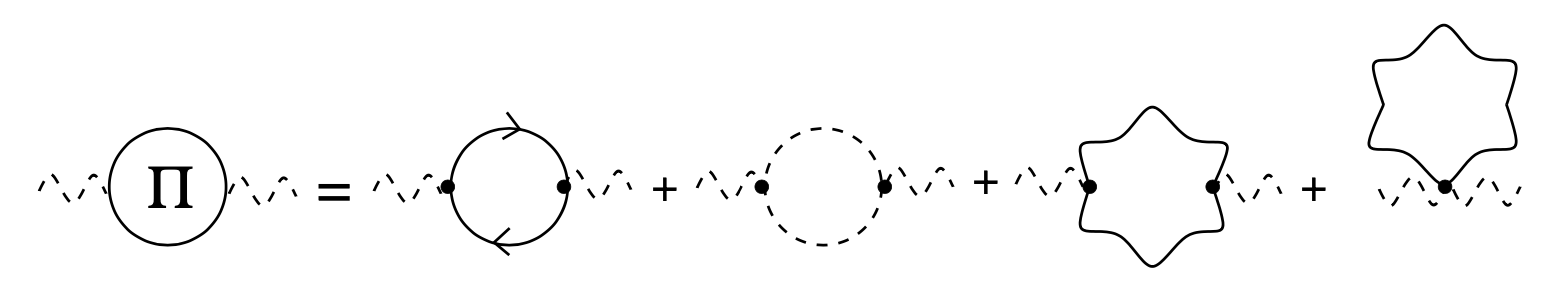
\includegraphics[width=.6\linewidth]{qcd_loop_propagator.png}
	\end{figure}
	
	\textbf{The ghost loop} is also similar, except now we have a factor of $N_c$ instead of $\frac{1}{2} N_f$, and with a frequency summation given by:
	\begin{equation}
	\begin{aligned}
		&\phantom{{}={}} \frac{T}{V} \sum_K
			\Delta(K)\,
				\pqty\big{-i\,(K-Q)^\nu}\,
			\Delta(K-Q)\,
				\pqty\big{-iK^\mu}, \quad
		\Delta(K) = \frac{1}{K^2} \\
		&= - \frac{T}{V} \sum_K
			\frac{(K-Q)^\nu K^\mu}{
				K^2 (K-Q)^2
			}
		\simeq - \frac{T}{V} \sum_K
			\frac{K^\mu K^\nu}{
				K^2 (K-Q)^2
			}
	\end{aligned}
	\end{equation}
	We've computed a similar Matsubara summation before, while treating the QED fermionic loop; the method still applies here but with bosonic frequencies. This produces an additional factor of $(-\frac{1}{8})$, relative to the fermionic case\footnote{
		Reference: Laine \& Vuorinen, \textit{Basics of Thermal Field Theory}. 
	}. In the end, we have:
	\begin{equation}
		m^2_E \longmapsto
		m^2_{\mrm{ghost}}\, \delta^{ab}
		= -\frac{1}{8} N_c\, \delta^{ab}
	\end{equation}
	
\printbibliography[%
%	title = {参考文献} %
	,heading = bibintoc
]
\end{document}
